\documentclass{beamer}
\usepackage{graphicx}
\usepackage{amsfonts}
\usepackage{amsmath}
\usepackage{amsthm}
\usepackage{amssymb}
\usepackage{calc}
\usepackage{hyperref}
\usepackage{float}
\setbeamertemplate{caption}[numbered]
\title{\textbf{\Huge Presentation of project 5}}
\author{Jose Emilio Ruiz Navarro}
\date{\today}
\institute{University of Oslo}
\begin{document}
	
	\frame{\titlepage}
	
	\begin{frame}
		\frametitle{Table of contents}
		\tableofcontents
		All the files are located here: \url{https://github.com/jeruiznavarro/FYS3150/tree/master/Project5}
	\end{frame}
	
	\section{Introduction}
	
		\subsection{What is it?}

			\begin{frame}{\secname : \subsecname}
				\begin{itemize}
					\item Molecular dynamics (MD) is a computational technique that can be used to simulate particle systems that interact with each other by means of a \textit{classical} force field.
					\item The exact trajectories of the particles are not important to calculate equilibrium and transport properties, and as long as the possible different microstates spawned by the variations in the initial conditions represent the same macrostate, the measurements won't be affected by chaotic effects.
					\item The original description given by Alder and Wainwright in 1957 was: ``The method consists of solving exactly (to the number of significant figures carried) the simultaneous classical equations of motion of several hundred particles by means of fast electronic computors.''\cite{alder} The simulations were run on an UNIVAC and an IBM-704, running programs written in machine code or FORTRAN I with up to $500$ hard sphere-like particles.
				\end{itemize}
			\end{frame}
			
		\subsection{Where it's used and where it should not be used}
		
			\begin{frame}{\secname : \subsecname}
				\begin{itemize}
					\item MD is quite popular in some biological fields like biophysics and biochemistry (useful for macromolecules like proteins, DNA, RNA, etc.).
					\item The topic of protein folding sees extensive use of MD and improvements on it could lead to great medical advances.
					\item There are also studies in other biological structures like membranes/layers or even small viruses\cite{virus}.
					\item It can be used in chemistry and physics as well (mainly statistical and solid state physics) to study complex molecules like fullerenes, to probe into transport phenomena (like diffusion in this work or adsorption), structural properties like the radial distribution function or defects, processes in solids like fracture and friction, etc, so it's an important tool.
				\end{itemize}
			\end{frame}
			
			\begin{frame}{\secname : \subsecname}
				There are obviously some limitations to MD:
				
				\begin{itemize}
					\item The systems that can be modelled are naturally chaotic, small differences in the initial conditions will grow exponentially with time. 
					\item There's also the problem of ergodicity, because time averaging is the main way to perform measurements.
					\item The interaction between the particles is crucial, without the appropriate force fields/potentials the results will be bad.
					\item Time and size are important constraints, without massively parallel computational power, a decently sized system can only be simulated for relatively short time scales in the order of the nanoseconds.
					\item Finally, everything is treated in a strictly classical approach, thus no quantum effects must be relevant in the systems to be simulated, like high frequency hydrogen bonds or very low temperatures.
				\end{itemize}
			\end{frame}
		 	
	\section{Theory and methods}
	
		\subsection{Potential}
		
			\begin{frame}{\secname : \subsecname}
				The potential that will be used for the Argon system is the standard Lennard-Jones potential that works on a pair of particles:
		
				\begin{equation}U\left(r_{ij}\right)=4\epsilon\left[\left(\frac{\sigma}{r_{ij}}\right)^{12}-\left(\frac{\sigma}{r_{ij}}\right)^6\right]=4\epsilon\left(\frac{\sigma}{r_{ij}}\right)^6\left[\left(\frac{\sigma}{r_{ij}}\right)^6-1\right]\end{equation}\
			
				%Where $\epsilon$ gives the dimensions of energy and controls the depth of the well and $\sigma$ represents the point where $U\left(r_{ij}\right)=0$. The negative term is responsible for the long-range attraction and has a physical basis on the behaviour of dipoles, while the positive term accounts for the short-range repulsion and has an exponent equal to $12$ for convenience as seen by the factorisation, but it has no physical meaning beyond accounting for the repulsion (other values are possible too, $9$ is also used in some situations).\\
			
				Then the forces will be given by the negative gradient of the potential:
		
				\begin{equation}\mathbf{F}\left(r_{ij}\right)=-\nabla_{ij}U\left(r_{ij}\right)=-\frac{\partial U\left(r_{ij}\right)}{\partial r_{ij}}\nabla_{ij}\mathbf{r}_{ij}=24\epsilon\left(\frac{\sigma}{r_{ij}}\right)^6\left[2\left(\frac{\sigma}{r_{ij}}\right)^6-1\right]\frac{\mathbf{r}_{ij}}{r_{ij}^2}\end{equation}
			\end{frame}
		
			\begin{frame}{\secname : \subsecname}
				\begin{itemize}
					\item Periodic boundary conditions must be used in the simulation to avoid surface effects being relevant. Typically, between $10\%$ and $1\%$ of the particles will be in the surface, so this is not a realistic circumstance.
					\item Each face of the simulation box is connected with the opposite one, so when a particle crosses one of the faces of the box it will appear on the opposite side of the system.
					\item The minimum image convention (or cell lists) can be used so that there is no problem when the particles interact with those on the opposite side of the system.
					\item To speed up the simulation and solve this problem at the same time cell and/or neighbour lists can be used, since interactions are very weak after a certain distance.
				\end{itemize}
			\end{frame}
			
			\begin{frame}{\secname : \subsecname}
				The potential looks like this:
				
				\begin{figure}[ht!]\begin{center}\includegraphics[scale=0.66]{lennard_jones.eps}\par\protect\caption{Standard 12-6 Lennard-Jones potential with $\sigma=1$ and $\epsilon=1$, the former controls the width of the potential well while the latter regulates the depth of the minimum.}\end{center}\end{figure}
			\end{frame}
		
		\subsection{Integrators}
		
			\begin{frame}{\secname : \subsecname}
				Knowing the forces (thus the accelerations), an integrator can be used to move the particles. An integrator is a numerical scheme that solves the equations of movement of a system. The simplest integrator is the Euler-Cromer one, it's defined by:
		
				\begin{equation*}\mathbf{v}\left(t+\Delta t\right)=\mathbf{v}\left(t\right)+\mathbf{a}\left(t\right)\Delta t\end{equation*}
		
				\begin{equation*}\mathbf{r}\left(t+\Delta t\right)=\mathbf{r}\left(t\right)+\mathbf{v}\left(t+\Delta t\right)\Delta t\end{equation*}
			\end{frame}
			
		\subsection{Integrators}
				
			\begin{frame}{\secname : \subsecname}
				The Velocity-Verlet integrator is defined by:
		
				\begin{equation*}\mathbf{v}\left(t+\Delta t/2\right)=\mathbf{v}\left(t\right)+\mathbf{a}\left(t\right)\frac{\Delta t}{2}\end{equation*}\\
		
				\begin{equation*}\mathbf{r}\left(t+\Delta t\right)=\mathbf{r}\left(t\right)+\mathbf{v}\left(t+\Delta t/2\right)\Delta t\end{equation*}\\
		
				\begin{equation*}\mathbf{v}\left(t+\Delta t\right)=\mathbf{v}\left(t+\Delta t/2\right)+\mathbf{a}\left(t+\Delta t\right)\frac{\Delta t}{2}\end{equation*}\\
				
				\begin{itemize}
					\item It's area-preserving in the phase space.
					\item It's also time-reversible, like Newton's or Hamilton's equations.
					\item Conserves energy quite well over long timescales.
					\item It's also very simple so it's the main integrator in MD programs. The Euler-Cromer integrator does not have the previous characteristics.
				\end{itemize}
			\end{frame}

		\subsection{Measuring properties}
		
			\begin{frame}{\secname : \subsecname}
				As for measurements, they must be a function of the positions and momenta of the particles. The temperature can be easily computed using the equipartition theorem and the direct calculation of the kinetic energy:
		
				\begin{equation*}\left\langle E_k\right\rangle=\frac{3}{2}Nk_BT\hspace{0.25 cm}\Rightarrow\hspace{0.25 cm}T=\frac{2E_k}{3Nk_B}=\frac{\sum_{i=1}^N{m_iv_i^2}}{3Nk_B}\end{equation*}
				
				To obtain the diffusion constant it suffices to calculate the mean square displacement defined as follows:
				
				\begin{equation*}\left\langle r^2\left(t\right)\right\rangle=6Dt\end{equation*}
		
				With $t$ being the time. For each individual atom it is defined as:
		
				\begin{equation*}r_i^2\left(t\right)=\left|\mathbf{r}_i\left(t\right)-\mathbf{r}_i\left(0\right)\right|^2\end{equation*}
				
				For more general details on MD see\cite{understanding} and for more on MD about argon see\cite{argon}.
			\end{frame}

		\subsection{Algorithm for the program}
		
			\begin{frame}{\secname : \subsecname}
				For the code, the general structure that all MD codes follow is conceptually very simple and similar to how an actual experiment is performed.
		
				\begin{itemize}
					\item First of all, the program needs the initial conditions like pressure or temperature, positions, speeds, masses, etc.
		
					\item Next, the system is initialised (removing global momentum of the system, minimising high-energy configurations if needed, etc.) and the forces are calculated, which is the most computationally intensive part.
		
					\item Then, the integration of the movement happens. This part is also intensive but not as much as the calculation of the forces because it scales as $\mathcal{O}\left(n\right)$ instead of $\mathcal{O}\left(n^2\right)$ like the force calculation.
		
					\item Finally, the appropriate measurements are taken.
					
					\item After all the previous steps, the next timestep starts and the program goes back to the force calculation until all the timesteps have been completed.
				\end{itemize}
			\end{frame}
		
			\begin{frame}{\secname : \subsecname}
				\begin{figure}[ht!]\begin{center}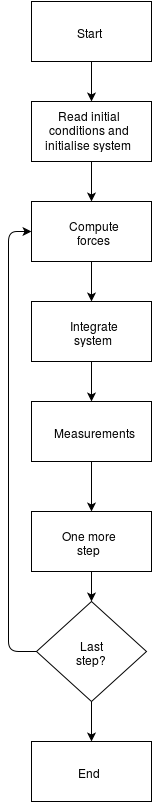
\includegraphics[scale=0.25]{MD.png}\par\protect\caption{General flow diagram of a molecular dynamics. program.}\end{center}\end{figure}
			\end{frame}
		
	\section{Results}

		\begin{frame}{\secname}
			\begin{itemize}
				\item The measured density of the system was $~0.0275$ atoms per cubic \AA, in a FCC lattice with a constant of $5.26$ \AA, which is equal to $\sim1.824$ times as dense as water, a reasonable value for solid Ar.
		
				\item The variance of the energy is a good measurement to compare both integrators:
			\end{itemize}
				
			\begin{figure}[ht!]\begin{center}\includegraphics[scale=0.5]{sigma_e.eps}\par\protect\caption{$\sigma_E$ vs. $\Delta t$ for two different temperatures.}\end{center}\end{figure}
		\end{frame}
		
		\begin{frame}{\secname}
			The conservation of energy is very good, and improves quite a lot when the timesteps become smaller:
			
			\begin{figure}[ht!]\begin{center}\includegraphics[scale=0.66]{energy_evolution.eps}\par\protect\caption{$E$ vs. $t$ for the Velocity-Verlet integrator.}\end{center}\end{figure}
		\end{frame}
		
		\begin{frame}{\secname}
			Here's a typical example of how the temperature decreases after some time from the initial and higher value:
			
			\begin{figure}[ht!]\begin{center}\includegraphics[scale=0.66]{temperature_evolution.eps}\par\protect\caption{$T$ vs. $t$ for the Velocity-Verlet integrator.}\end{center}\end{figure}
		\end{frame}
		
		\begin{frame}{\secname}
			To estimate the melting temperature, the diffusion measurements can be used since the diffusion constant will be very small in the solid state:
		
			\begin{figure}[ht!]\begin{center}\includegraphics[scale=0.5]{diffusion.eps}\par\protect\caption{$D$ vs. $T$, the clear increase shows the system melting.}\end{center}\end{figure}
		\end{frame}
		
	\section{Conclusions}
	
		\begin{frame}{\secname}
			\begin{itemize}
				\item The Velocity-Verlet integrator is the best one. For the smallest values of the timestep, the difference is about three orders of magnitude for the standard deviation of the total energy, and even for the highest timestep the difference is more than one order of magnitude. The energy drift is also very small.
				\item The decrease in the temperature at the beginning is due to the exchange between kinetic energy and potential energy because a perfect lattice is not a realistic initial condition. The system will be far away from equilibrium and it will try to become as stable as possible.
				\item The ratio between the final and initial temperatures is usually a bit less than $1/2$, but can be as low as $1/3$ for higher temperatures. This is because higher initial temperatures make configurations with high potential energy more likely.
			\end{itemize}
		\end{frame}
		
		\begin{frame}{\secname}
			\begin{itemize}
				\item There is a sharp increase in the value of the diffusion constant in a very small temperature interval. This allows for the estimation of the melting temperature of the system as it goes from solid to liquid. Since the increase is very sudden between $280$ and $290$ K, a tentative value of $285\pm5$ K is a reasonable choice.
				\item The diffusion constant remains practically the same for a wide range of temperatures before the phase transition happens, because the particles in a solid will oscillate around fixed equilibrium positions.
			\end{itemize}
		\end{frame}
	
		%In the future, it would be interesting to try using a parallel approach to the program so that bigger systems could be simulated (or the same systems being simulated for a longer period of time). More complex schemes like cells list or neighbour lists could be used to improve the efficiency of the force calculation function of the program, which is the main bottleneck towards faster computation. Trying to use other force fields would enable the possibility of simulating molecules instead of simple atoms (although this requires a much more complex program). Finally, there are other physical properties of interest that could be measured without much effort, like pressure or the radial structure function.\\
	
		%As for the didactic value of the project, I would personally say that it was a very valuable introduction to object orientated programming. Above the physical topics covered, I feel this is the most important lesson learnt in this case, because it provides a nice way to start learning how to deal with classes and objects in general. From a more physical point of view, it is a nice way to get a different view of statistical mechanics and thermodynamics in general, since it offers the possibility of ``playing'' with a system and ``seeing'' what happens with it constituent parts. It also exposes the student to some not-so-famous physical topics (compared to the Ising model or the initial numerical exercises) like the different integrators or the Lennard-Jones potential.\\
		
	\section{Bibliography}
		
		\begin{frame}{\secname}
			\bibliographystyle{abbrv}
			\bibliography{bibliography.bib}
		\end{frame}
		
\end{document}